\documentclass[10pt]{article}
\usepackage[a4paper,margin=18mm]{geometry}
\usepackage{amsmath,amssymb,booktabs,array,enumitem}
\usepackage[T1]{fontenc}\usepackage{lmodern}
\usepackage{tikz}\usetikzlibrary{shapes.gates.logic.US,positioning,arrows.meta}
\usepackage[hidelinks]{hyperref}
\setlength{\parindent}{0pt}\setlength{\parskip}{4pt}
\setlength{\emergencystretch}{2em}
\newcommand{\VDD}{V_{DD}}
\newcommand{\mos}[4]{\begin{scope}[shift={(#1,#2)}]
\draw (0,.24)--(0,-.24);\draw (0,.20)--(.25,.20)--(.25,.5);
\draw (0,-.20)--(.25,-.20)--(.25,-.5);\draw (-.16,.23)--(-.16,-.23);
\ifnum#4=1\draw (-.26,0) circle (.06);\draw (-.75,0)--(-.32,0);\else\draw (-.75,0)--(-.16,0);\fi
\node[anchor=east,font=\scriptsize] at (-.76,0) {$#3$};\end{scope}}
\newcommand{\ground}[2]{\draw (#1,#2)--(#1,{#2-.12});\draw ({#1-.17},{#2-.12})--({#1+.17},{#2-.12});\draw ({#1-.11},{#2-.20})--({#1+.11},{#2-.20});}
\newcommand{\rail}[3]{\draw (#1,#2)--(#1,{#2+.14});\node[above,font=\scriptsize] at (#1,{#2+.14}) {$#3$};}
\begin{document}
\begin{center}{\large\bfseries EE3032 Introduction to VLSI -- Midterm}\end{center}
\textbf{1. (30 points)} Answer the following questions briefly.
\begin{enumerate}[label=(\alph*),leftmargin=7mm,itemsep=2pt,topsep=2pt]
\item Increasing the supply voltage of a CMOS circuit can boost the operation speed of the CMOS circuit. However, the designer typically doesn't use this approach. Why? (4 points)
\item List the process for transferring the mask pattern to the surface of a silicon region. (3 points)
\item Explain how to tune the size of FinFET transistors. (2 points)
\item List two features of static CMOS circuits. (2 points)
\item A CMOS circuit consumes static power caused by two static currents. List the two static currents. (2 points)
\item List the steps of chip-on-wafer assembly process for integrating a die on an interposer. (5 points)
\item Explain the back-side power supply technology and list its two advantages. (4 points)
\item In a CMOS gate, the transistors connected to the gate output suffer from the severest body effect. Why? (2 points)
\item Switching speed of a MOS transistor depends on multiple parameters. List the parameters. (3 points)
\item The output capacitance of a CMOS logic gate in a CMOS circuit is comprised of three components. List the three components. (3 points)
\end{enumerate}
\textbf{2. (15 points)} Fig. 1 shows a multiplexer-based circuit. (a) Complete the circuit such that it realizes the Boolean functions $f(x,y,z)=xy+yz$ and $f(x,y,z)=x+y+z$ when $s=1$ and $s=0$, respectively. (10 points) (b) If the 2-to-1 multiplexer is realized by transmission gates without buffer insertion, express the delay of the circuit in terms of the number of multiplexer stages. Explain your answer. (5 points)
\begin{center}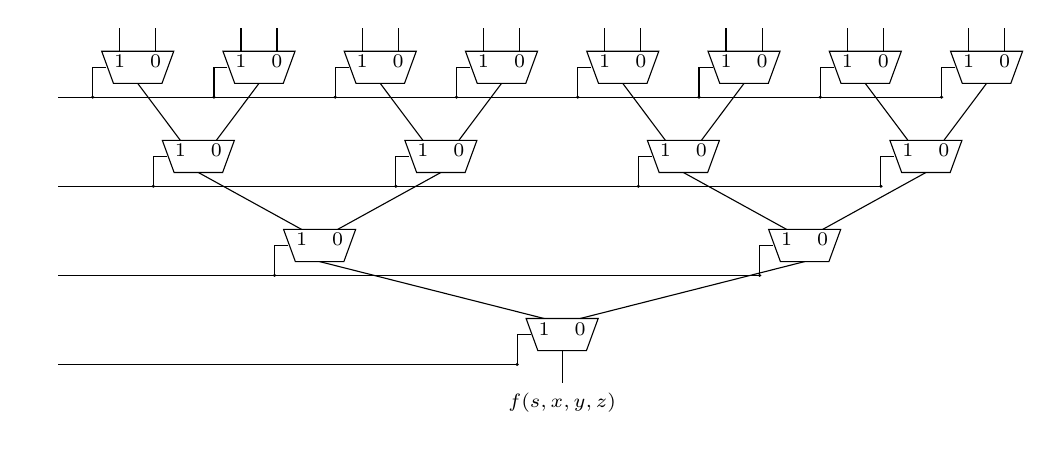
\begin{tikzpicture}[x=.88cm,y=.73cm,font=\scriptsize]
\draw (-0.520,3.280)--(0.520,3.280)--(0.350,2.720)--(-0.350,2.720)--cycle;
\node at (-0.260,3.100) {1};\node at (0.260,3.100) {0};
\draw (-0.260,3.280)--(-0.260,3.680);
\draw (0.260,3.280)--(0.260,3.680);
\draw (1.230,3.280)--(2.270,3.280)--(2.100,2.720)--(1.400,2.720)--cycle;
\node at (1.490,3.100) {1};\node at (2.010,3.100) {0};
\draw (1.490,3.280)--(1.490,3.680);
\draw (2.010,3.280)--(2.010,3.680);
\draw (2.980,3.280)--(4.020,3.280)--(3.850,2.720)--(3.150,2.720)--cycle;
\node at (3.240,3.100) {1};\node at (3.760,3.100) {0};
\draw (3.240,3.280)--(3.240,3.680);
\draw (3.760,3.280)--(3.760,3.680);
\draw (4.730,3.280)--(5.770,3.280)--(5.600,2.720)--(4.900,2.720)--cycle;
\node at (4.990,3.100) {1};\node at (5.510,3.100) {0};
\draw (4.990,3.280)--(4.990,3.680);
\draw (5.510,3.280)--(5.510,3.680);
\draw (6.480,3.280)--(7.520,3.280)--(7.350,2.720)--(6.650,2.720)--cycle;
\node at (6.740,3.100) {1};\node at (7.260,3.100) {0};
\draw (6.740,3.280)--(6.740,3.680);
\draw (7.260,3.280)--(7.260,3.680);
\draw (8.230,3.280)--(9.270,3.280)--(9.100,2.720)--(8.400,2.720)--cycle;
\node at (8.490,3.100) {1};\node at (9.010,3.100) {0};
\draw (8.490,3.280)--(8.490,3.680);
\draw (9.010,3.280)--(9.010,3.680);
\draw (9.980,3.280)--(11.020,3.280)--(10.850,2.720)--(10.150,2.720)--cycle;
\node at (10.240,3.100) {1};\node at (10.760,3.100) {0};
\draw (10.240,3.280)--(10.240,3.680);
\draw (10.760,3.280)--(10.760,3.680);
\draw (11.730,3.280)--(12.770,3.280)--(12.600,2.720)--(11.900,2.720)--cycle;
\node at (11.990,3.100) {1};\node at (12.510,3.100) {0};
\draw (11.990,3.280)--(11.990,3.680);
\draw (12.510,3.280)--(12.510,3.680);
\draw (-1.15,2.480)--(11.600,2.480);\node[left] at (-1.15,2.480) {$\phantom{z}$};
\draw (-0.650,2.480)--(-0.650,3.0)--(-0.455,3.0);\fill (-0.650,2.480) circle (.027);
\draw (1.100,2.480)--(1.100,3.0)--(1.295,3.0);\fill (1.100,2.480) circle (.027);
\draw (2.850,2.480)--(2.850,3.0)--(3.045,3.0);\fill (2.850,2.480) circle (.027);
\draw (4.600,2.480)--(4.600,3.0)--(4.795,3.0);\fill (4.600,2.480) circle (.027);
\draw (6.350,2.480)--(6.350,3.0)--(6.545,3.0);\fill (6.350,2.480) circle (.027);
\draw (8.100,2.480)--(8.100,3.0)--(8.295,3.0);\fill (8.100,2.480) circle (.027);
\draw (9.850,2.480)--(9.850,3.0)--(10.045,3.0);\fill (9.850,2.480) circle (.027);
\draw (11.600,2.480)--(11.600,3.0)--(11.795,3.0);\fill (11.600,2.480) circle (.027);
\draw (0.355,1.730)--(1.395,1.730)--(1.225,1.170)--(0.525,1.170)--cycle;
\node at (0.615,1.550) {1};\node at (1.135,1.550) {0};
\draw (0.000,2.720)--(0.615,1.730);
\draw (1.750,2.720)--(1.135,1.730);
\draw (3.855,1.730)--(4.895,1.730)--(4.725,1.170)--(4.025,1.170)--cycle;
\node at (4.115,1.550) {1};\node at (4.635,1.550) {0};
\draw (3.500,2.720)--(4.115,1.730);
\draw (5.250,2.720)--(4.635,1.730);
\draw (7.355,1.730)--(8.395,1.730)--(8.225,1.170)--(7.525,1.170)--cycle;
\node at (7.615,1.550) {1};\node at (8.135,1.550) {0};
\draw (7.000,2.720)--(7.615,1.730);
\draw (8.750,2.720)--(8.135,1.730);
\draw (10.855,1.730)--(11.895,1.730)--(11.725,1.170)--(11.025,1.170)--cycle;
\node at (11.115,1.550) {1};\node at (11.635,1.550) {0};
\draw (10.500,2.720)--(11.115,1.730);
\draw (12.250,2.720)--(11.635,1.730);
\draw (-1.15,0.930)--(10.725,0.930);\node[left] at (-1.15,0.930) {$\phantom{z}$};
\draw (0.225,0.930)--(0.225,1.45)--(0.420,1.45);\fill (0.225,0.930) circle (.027);
\draw (3.725,0.930)--(3.725,1.45)--(3.920,1.45);\fill (3.725,0.930) circle (.027);
\draw (7.225,0.930)--(7.225,1.45)--(7.420,1.45);\fill (7.225,0.930) circle (.027);
\draw (10.725,0.930)--(10.725,1.45)--(10.920,1.45);\fill (10.725,0.930) circle (.027);
\draw (2.105,0.180)--(3.145,0.180)--(2.975,-0.380)--(2.275,-0.380)--cycle;
\node at (2.365,-0.000) {1};\node at (2.885,-0.000) {0};
\draw (0.875,1.170)--(2.365,0.180);
\draw (4.375,1.170)--(2.885,0.180);
\draw (9.105,0.180)--(10.145,0.180)--(9.975,-0.380)--(9.275,-0.380)--cycle;
\node at (9.365,-0.000) {1};\node at (9.885,-0.000) {0};
\draw (7.875,1.170)--(9.365,0.180);
\draw (11.375,1.170)--(9.885,0.180);
\draw (-1.15,-0.620)--(8.975,-0.620);\node[left] at (-1.15,-0.620) {$\phantom{z}$};
\draw (1.975,-0.620)--(1.975,-0.10000000000000009)--(2.170,-0.10000000000000009);\fill (1.975,-0.620) circle (.027);
\draw (8.975,-0.620)--(8.975,-0.10000000000000009)--(9.170,-0.10000000000000009);\fill (8.975,-0.620) circle (.027);
\draw (5.605,-1.370)--(6.645,-1.370)--(6.475,-1.930)--(5.775,-1.930)--cycle;
\node at (5.865,-1.550) {1};\node at (6.385,-1.550) {0};
\draw (2.625,-0.380)--(5.865,-1.370);
\draw (9.625,-0.380)--(6.385,-1.370);
\draw (-1.15,-2.170)--(5.475,-2.170);\node[left] at (-1.15,-2.170) {$\phantom{z}$};
\draw (5.475,-2.170)--(5.475,-1.6500000000000004)--(5.670,-1.6500000000000004);\fill (5.475,-2.170) circle (.027);
\draw (6.125,-1.9300000000000004)--(6.125,-2.5000000000000004) node[below] {$f(s,x,y,z)$};
\end{tikzpicture}\end{center}\begin{center}\small Figure 1: A multiplexer-based circuit.\end{center}
\textbf{3. (10 points)} Fig. 2 shows a CMOS circuit driving a load capacitance $C_L=C$. The inverter A is a minimum-size inverter (the size of NMOS and PMOS is $W/L$) and its input capacitance is $C_g$. Assumptions: 1) the drain and wire parasitic capacitance can be neglected; 2) $e\simeq2.7$, $e^2\simeq7.2$, $e^3\simeq20$, and $e^4\simeq54$; 3) $\mu_p=\mu_n$; 4) the turn-on resistance of a PMOS transistor with $W/L$ is $R$. If the simple RC model is used to estimate the delay such that the output rise time $t_r$ of the NAND gate D is $0.05RC$, design the buffer shown in dash such that delay time $T$ is minimized.

\textbf{4. (10 points)} Fig. 3(a) shows a CMOS logic gate. Assume that the threshold voltage of the NMOS transistor is 0.4 V; the turn-on resistance of N1, N2, and N3 is $R$, $2R$, and $R$, respectively. If the initial voltage of the output $V_{out}$ is 1.2 V and an input stimulus (0--1.2) shown in Fig. 3(b) is applied, (a) how much voltage of the input stimulus at $x$? (4 points) (b) Identify the operation region of the transistors N1, N2, and N3 from $t_1$ to $t_2$. (6 points)
\newpage
\begin{center}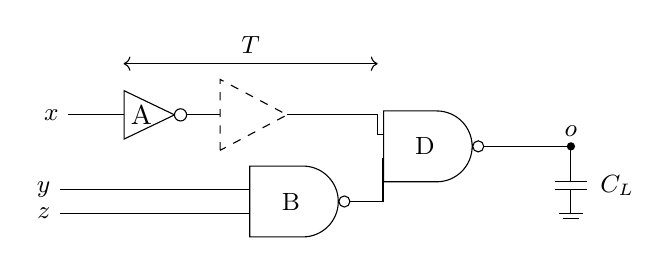
\begin{tikzpicture}[font=\small]
\node[not gate US,draw,scale=1.1] (A) at (0,1) {A};
\draw (A.input)--++(-.7,0) node[left]{$x$};
\draw[dashed] (1, .55)--(1,1.45)--(1.85,1)--cycle;
\draw (A.output)--(1,1);\draw (1.85,1)--(3,1);
\node[nand gate US,draw,logic gate inputs=nn,logic gate input sep=.3cm] (D) at (3.6,.6) {D};
\draw (3,1)|-(D.input 1);
\node[nand gate US,draw,logic gate inputs=nn,logic gate input sep=.3cm] (B) at (1.9,-.1) {B};
\draw (B.input 1)--++(-2.4,0) node[left]{$y$};\draw (B.input 2)--++(-2.4,0) node[left]{$z$};
\draw (B.output)-|(D.input 2);\draw (D.output)--++(1.1,0) coordinate(o) node[above]{$o$};
\fill(o) circle(1.5pt);\draw(o)--++(0,-.45);\draw([yshift=-.45cm]o)++(-.2,0)--++(.4,0);
\draw([yshift=-.55cm]o)++(-.2,0)--++(.4,0);\draw([yshift=-.55cm]o)--++(0,-.3);\draw([yshift=-.85cm]o)++(-.15,0)--++(.3,0);\draw([yshift=-.92cm]o)++(-.10,0)--++(.2,0);\node[right] at ([xshift=.25cm,yshift=-.5cm]o) {$C_L$};
\draw[<->] (A.input)+(0,.65)--(3,1.65) node[midway,above]{$T$};
\end{tikzpicture}\end{center}\begin{center}\small Figure 2: A simple CMOS circuit.\end{center}
\begin{center}\begin{tikzpicture}[font=\small]
\draw[dashed](-.1,3.25) rectangle (1.5,4.25);\node[align=center] at(.7,3.75){p\ network};\rail{.7}{4.25}{1.2\,\mathrm V}
\draw(.7,3.25)--(.7,2.5);\mos{.45}{2}{}{0}\mos{.45}{.6}{}{0}\node[right]at(.95,2){N3};\node[right]at(.95,.6){N1};
\draw(.7,1.5)--(.7,1.1);\ground{.7}{.1}
\draw(-.9,.6)--(-.9,2)--(-.3,2);\draw(-.9,.6)--(-.3,.6);\draw(-1.6,1.3)--(-.9,1.3) node[pos=0,left]{$V_{in}$};
\draw(.7,2.75)--(2.8,2.75) node[right]{$V_{out}$};\fill(.7,2.75) circle(1.5pt);
% N2 horizontal: channel .6cm above common junction, gate tied to output.
\draw(1.9,1.55)--(2.4,1.55);\draw(1.9,1.55)--(1.9,1.3)--(.7,1.3);\fill(.7,1.3)circle(1.5pt);
\draw(2.4,1.55)--(2.4,1.3)--(3.0,1.3) node[right]{$1.2\,\mathrm V$};
\draw(1.95,1.75)--(2.35,1.75);\draw(2.15,1.75)--(2.15,2.75);\fill(2.15,2.75) circle(1.5pt);\node at(2.15,.95){N2};
\node at(.7,-.5){(a)};
\begin{scope}[shift={(5.2,.4)},x=1.2cm,y=2.2cm]
\draw[->](0,0)--(2.35,0) node[right]{time};\draw[->](0,0)--(0,1.65) node[above]{Voltage};
\draw(0,1.2)--(1.2,1.2)--(1.65,0);\node at(.55,1.36){$V_{out}$};
\draw(0,0)--(1.8,1.2)--(2.12,1.2);\node at(2.02,1.42){$V_{in}$};
\draw[dashed](0,.4)--(.6,.4)--(.6,0);\draw[dashed](0,.8)--(1.2,.8)--(1.2,0);
\node[left]at(0,1.2){1.2 V};\node[left]at(0,.4){0.4 V};
\node[below]at(.6,0){$t_1$};\node[below]at(1.2,0){$t_2$};\node[above left]at(1.2,.8){$x$};
\node at(1,-.35){(b)};
\end{scope}
\end{tikzpicture}\end{center}\begin{center}\small Figure 3: (a) A CMOS logic gate (b) waveforms of $V_{in}$ and $V_{out}$.\end{center}
\textbf{5. (10 points)} Fig. 4(a) shows a CMOS circuit. Assume that the sizes of NMOS and PMOS transistors in the logic gates are $W/L$ and $2W/L$, respectively. Also assume that $\mu_n=2\mu_p$. If the functional inputs of the circuits are $(ABCD)=\{0011,0101,1101,1001\}$, explain the relationship of noise margins $NM_L$ and $NM_H$ (i.e., $NM_L>NM_H$, $NM_L<NM_H$, or $NM_L=NM_H$) of the gates G2 and G3.
\begin{center}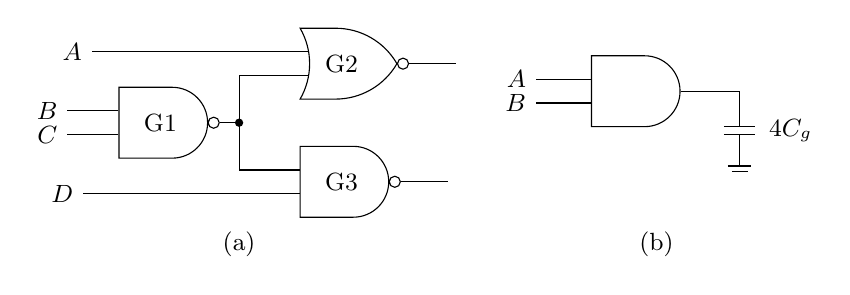
\begin{tikzpicture}[font=\small]
\node[nand gate US,draw,logic gate inputs=nn,logic gate input sep=.3cm] (G1) at(0,0){G1};
\node[nor gate US,draw,logic gate inputs=nn,logic gate input sep=.3cm] (G2) at(2.3,.75){G2};
\node[nand gate US,draw,logic gate inputs=nn,logic gate input sep=.3cm] (G3) at(2.3,-.75){G3};
\draw(G1.input 1)--++(-.65,0) node[left]{$B$};\draw(G1.input 2)--++(-.65,0) node[left]{$C$};
\draw(G1.output)--(1,0);\fill(1,0) circle(1.5pt);\draw(1,0)|-(G2.input 2);\draw(1,0)|-(G3.input 1);
\draw(G2.input 1)--++(-2.75,0) node[left]{$A$};\draw(G3.input 2)--++(-2.75,0) node[left]{$D$};
\draw(G2.output)--++(.6,0);\draw(G3.output)--++(.6,0);\node at(1,-1.55){(a)};
\node[and gate US,draw,logic gate inputs=nn,logic gate input sep=.3cm] (G) at(6,.4){};
\draw(G.input 1)--++(-.7,0) node[left]{$A$};\draw(G.input 2)--++(-.7,0) node[left]{$B$};
\draw(G.output)--++(.75,0) coordinate(load);\draw(load)--++(0,-.45);
\draw([yshift=-.45cm]load)++(-.2,0)--++(.4,0);\draw([yshift=-.55cm]load)++(-.2,0)--++(.4,0);
\draw([yshift=-.55cm]load)--++(0,-.4);\draw([yshift=-.95cm]load)++(-.15,0)--++(.3,0);\draw([yshift=-1.02cm]load)++(-.1,0)--++(.2,0);\node[right]at([xshift=.25cm,yshift=-.5cm]load){$4C_g$};\node at(6.3,-1.55){(b)};
\end{tikzpicture}\end{center}\begin{center}\small Figure 4: CMOS circuits.\end{center}
\textbf{6. (10 points)} For a given technology, the turn-on resistance of a $W/L$ NMOS is $R$ and $\mu_n=2\mu_p$. Also, the gate capacitance of a $W/L$ NMOS or PMOS transistor is $C_g$. Fig. 4(b) shows a two-input AND gate driving a $4C_g$ capacitive load. Design the AND gate such that the worst-case delay of the AND gate is smaller than $8RC_g$, where the delay is estimated by using simple RC model and the parasitic capacitance can be ignored. Draw the transistor-level schematic diagram and label the size of each transistor in terms of $W/L$.

\textbf{7. (15 points)} Realize the following Boolean functions using CMOS logic design style.
\[
\text{(a) }F=\overline{X(Y+Z)}\quad(5\text{ points})\qquad
\text{(b) }F=\overline{XY+Z}\quad(5\text{ points})
\]
\[\text{(c) }F=\overline{X+Y(W+Z)}\quad(5\text{ points}).\]
\vfill\small Li, EE, NCU. Typeset transcription of the supplied 2024 archive scan. All figures are editable vectors. Handwritten annotations are excluded; equations and circuit connectivity are preserved.
\end{document}
